% !TEX root = ../main.tex
%--- Slide 9: processi non modellati (circa 1 min 45 s) -----------------------------------
% Una sola slide ripetuta 3 volte (overlay 1, 2, 3): cambia il caso evidenziato e la figura.
% Figure: Figure/P09_1_GWB.pdf, P09_2_band.pdf, P09_3_GWB_band.pdf (notebook 26).
% Colori: dati reali blu, simulazione di riferimento arancione, nuova simulazione viola.
\begin{frame}{Processi presenti nei dati ma non nel modello}
  \setbeamercovered{transparent=25}
  \begin{columns}[c]
    \column{0.53\textwidth}\small
    Simulazioni con un processo in più, analizzate con il modello a 6 parametri
    \vspace{0.5mm}

    \uncover<1>{%
    \textbf{GWB} ($\log_{10}\Agwb$ da $-15.5$ a $-14.5$)
    \begin{itemize}\setlength{\itemsep}{0pt}
      \item Il red noise intrinseco cambia poco
      \item Deboli code a L, solo nei contorni al 99.7\%
    \end{itemize}}
    \vspace{0.5mm}

    \uncover<2>{%
    \textbf{Band noise} ($\log_{10}A_{\rm BN} = -12.5$)
    \begin{itemize}\setlength{\itemsep}{0pt}
      \item DM verso ampiezza alta e indice basso: zona del picco alto dei dati reali
      \item Ma un solo picco, niente L
    \end{itemize}}
    \vspace{0.5mm}

    \uncover<3>{%
    \textbf{GWB + band noise} ($-14$ e $-12.5$)
    \begin{itemize}\setlength{\itemsep}{0pt}
      \item DM spostato come con il solo band noise; red noise più forte e ripido
      \item Ma un solo picco, niente L
    \end{itemize}}
    \column{0.45\textwidth}
    \centering
    \only<1>{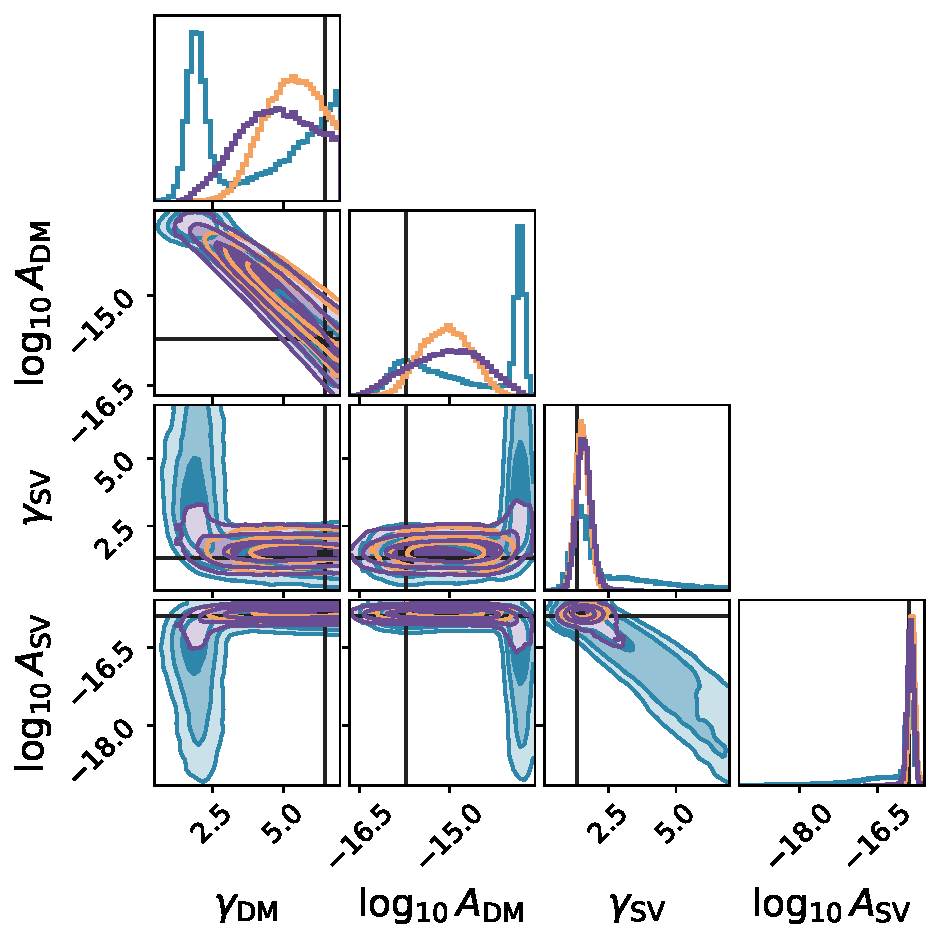
\includegraphics[height=0.66\textheight]{Figure/P09_1_GWB.pdf}}%
    \only<2>{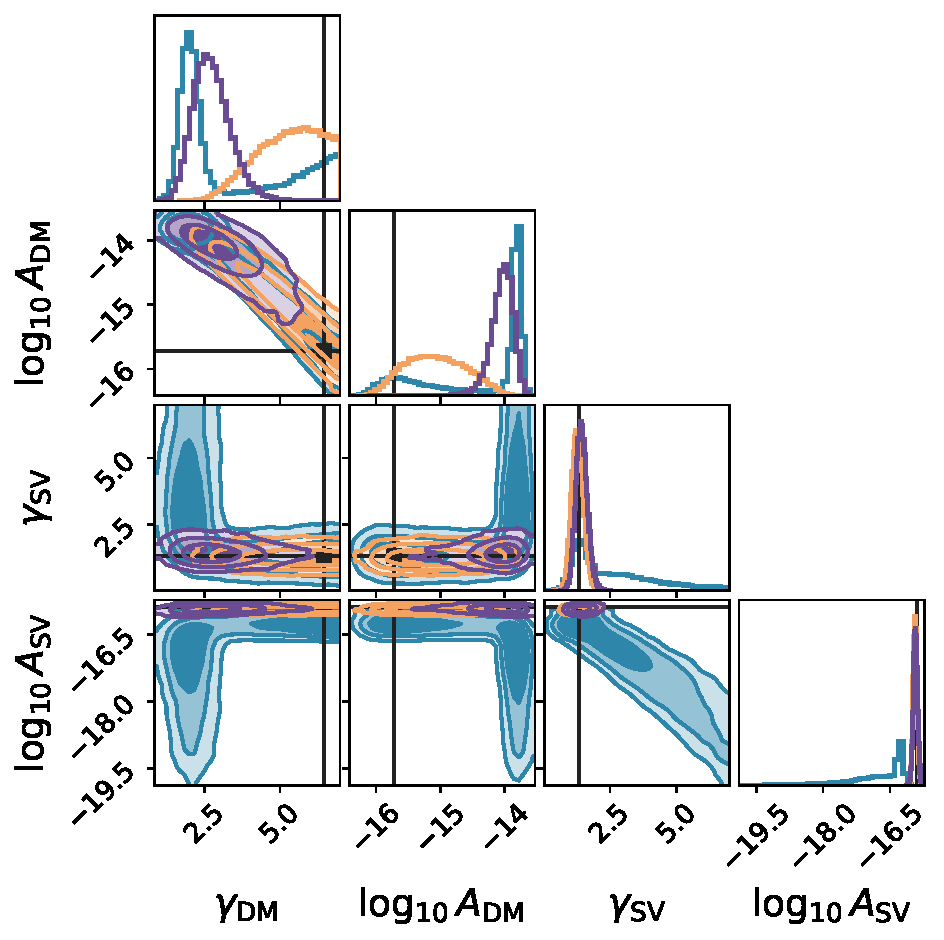
\includegraphics[height=0.66\textheight]{Figure/P09_2_band.pdf}}%
    \only<3>{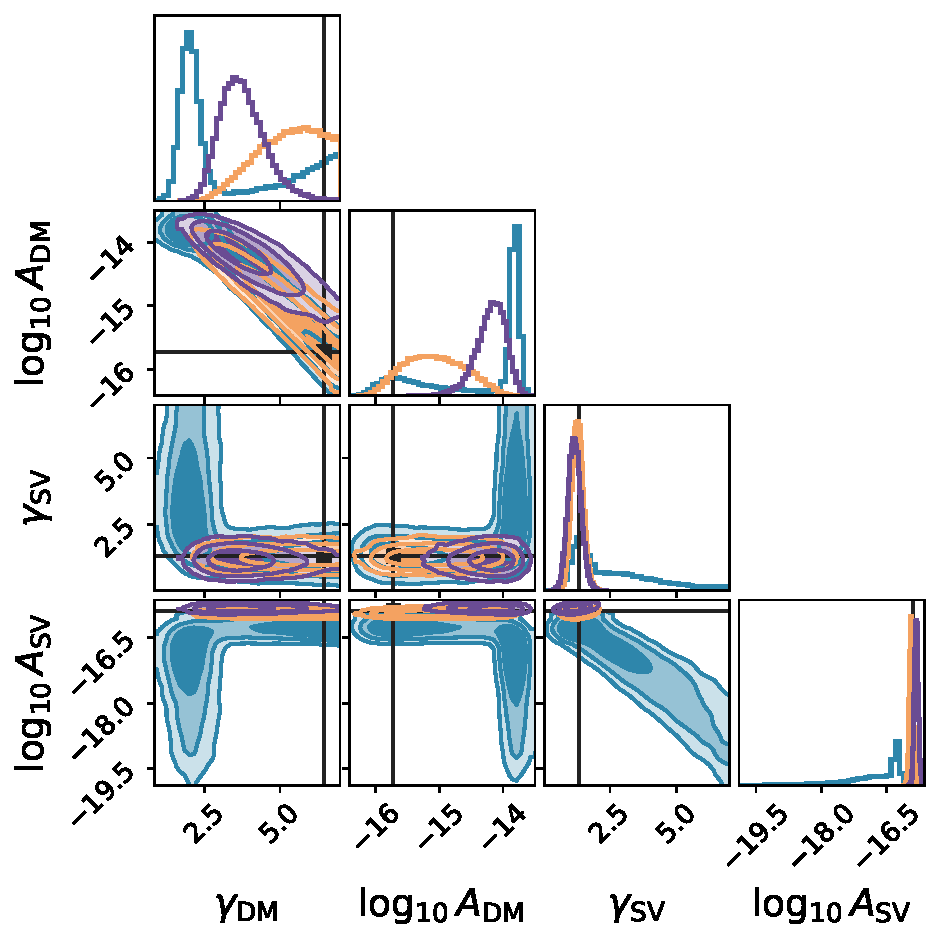
\includegraphics[height=0.66\textheight]{Figure/P09_3_GWB_band.pdf}}\par
    {\footnotesize \reali{dati reali} \quad \simul{riferimento} \quad
     \textcolor{simdue}{nuova simulazione}\\
     linee nere: valori iniettati}
  \end{columns}
\end{frame}
